\section{Flood Reporting as an Information Problem}

Flood reporting is an information problem before it is a software problem. The earliest signals of a flooded road or a blocked route usually come from people already near the affected area. These field observations arrive quickly, but they arrive in formats that are hard to reuse: a photo without a clear address, a short message without coordinates, or a location pin without enough context to judge severity. As a result, valuable information can be lost in message streams or become difficult to verify and track over time.

VietFlood follows the idea that citizen-generated information can support crisis response when it is organized into usable data. Research on crowdsourcing and crisis information highlights that local observations can provide timely coverage, but they require structure and processing to become useful in practice \cite{goodchild2010crowdsourcing,imran2015processing}. In this thesis, a ``report'' is treated as a durable record with fields that support review: what happened, where it happened, who reported it, what evidence exists, and what the current status is.

\subsection{Review States and Follow-Up}

The simplest trust signal in a reporting platform is the review status. VietFlood uses a small status set suitable for a prototype: \texttt{pending}, \texttt{verified}, \texttt{resolved}, and \texttt{rejected}. A new submission is pending. An administrator can mark it verified after review, resolved when it is no longer active, or rejected when the report is incorrect or unsuitable. Keeping rejected reports separate supports accountability by preserving the record of what was submitted rather than silently discarding it.

\begin{figure}[htbp]
    \centering
    \IfFileExists{images/figure2-1-report-lifecycle.png}{
        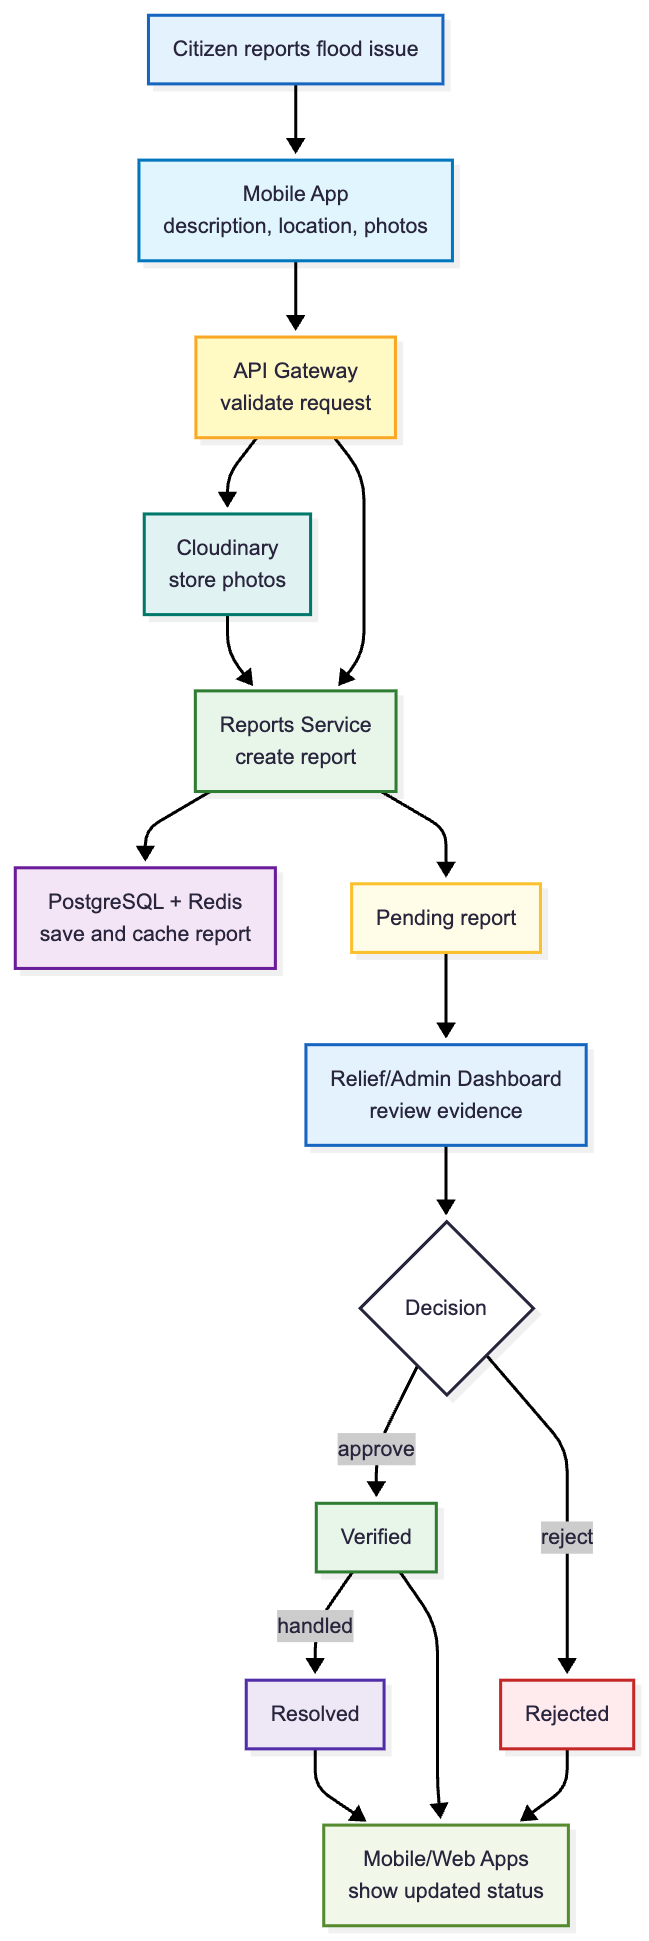
\includegraphics[width=1\linewidth,height=0.9\textheight,keepaspectratio]{images/figure2-1-report-lifecycle.png}
    }{
        \fbox{
            \begin{minipage}[c][4.8cm][c]{0.86\linewidth}
                \centering
                Placeholder for Figure 2.1\\[0.4cm]
                Suggested image: citizen creates report, gateway receives it, reports service stores it, reviewer changes status, dashboard shows updated case.\\[0.3cm]
                File name: \texttt{images/figure2-1-report-lifecycle.png}
            \end{minipage}
        }
    }
    \caption{VietFlood report flow from mobile submission to administrator review status.}
    \label{fig:chapter2-report-lifecycle}
\end{figure}

Figure~\ref{fig:chapter2-report-lifecycle} summarizes the report lifecycle used in the prototype. The purpose of the lifecycle is not to model every possible response action. Its purpose is to ensure that reports remain visible and reviewable after the initial submission, with a status that can be updated as more information becomes available.

\subsection{Mobile Reporting Constraints}

Reporting is expected to happen in the field, so mobile interaction is central. A mobile-first flow prioritizes short forms, simple location entry, and optional evidence upload rather than requiring long text input. VietFlood uses Expo React Native for the citizen and relief clients \cite{expoDocs,reactNativeDocs}. To reduce inconsistent spelling of administrative locations, the system uses the Vietnam Provinces Open API as a structured source for provinces and wards \cite{vietnamProvincesOpenApi}. This choice improves filterability and reduces ambiguity when multiple users describe the same area differently.

\section{Research Context and Key Concepts}

\subsection{Citizen Signals in Emergencies}

Two streams of related work motivate VietFlood. The first is crowdsourcing and volunteered geographic information in disasters. Goodchild and Glennon describe crowdsourcing geographic information as a research frontier in disaster response, highlighting both its potential value and the need for methods that transform observations into usable information products \cite{goodchild2010crowdsourcing}. The second is crisis communication through social media and messaging. Imran et al.\ survey methods for processing emergency-related social media messages and emphasize the challenges of noise, duplication, and incomplete context \cite{imran2015processing}. VietFlood does not attempt automated social media extraction, but it is designed to address the same practical problem: field information arrives quickly and inconsistently, and needs structure to support review.

\subsection{Responsibility-Driven Architecture}

The background for VietFlood's implementation is software architecture that makes responsibilities explicit. Architectural guidance emphasizes designing system structure around responsibilities and quality attributes, rather than only selecting technologies \cite{bass2021softwareArchitecture}. For this thesis, the most important responsibilities are: (1) public API handling and access control, (2) authentication and session management, (3) report persistence and status updates, and (4) evidence upload and retrieval. The design should also remain operable as a small prototype without a complex production platform.

\section{Backend Decomposition Options}

A single monolithic backend can be an effective approach for small projects. However, as features accumulate, authentication, file upload handling, report persistence, caching, and real-time communication can become tightly coupled. Microservice architecture is often defined as decomposing a system into services around capabilities, trading increased operational complexity for clearer boundaries and independent evolution \cite{fowlerLewis2014microservices,dragoni2017microservices,thones2015microservices}.

VietFlood adopts a modest service split suitable for a thesis prototype. The system uses an API gateway as the client-facing entry point, and internal services for authentication and report management. Supporting infrastructure (RabbitMQ, Redis, PostgreSQL, Cloudinary) is introduced only when it directly supports a needed responsibility.

\begin{figure}[htbp]
    \centering
    \IfFileExists{images/figure2-2-microservices-comparison.png}{
        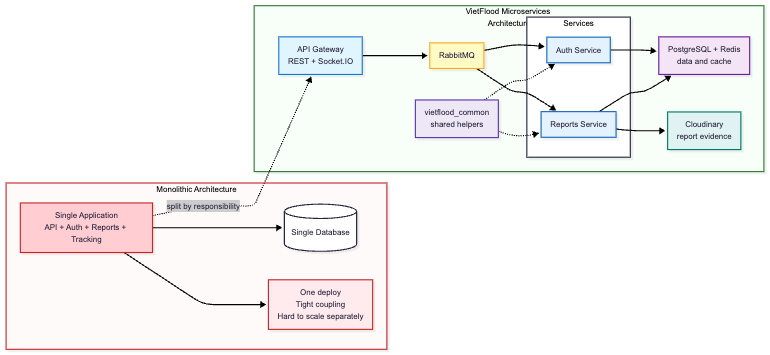
\includegraphics[width=0.9\linewidth,height=0.48\textheight,keepaspectratio]{images/figure2-2-microservices-comparison.png}
    }{
        \fbox{
            \begin{minipage}[c][5.2cm][c]{0.9\linewidth}
                \centering
                Placeholder for Figure 2.2\\[0.4cm]
                Suggested image: compare one monolithic backend with the VietFlood split of API gateway, auth service, reports service, RabbitMQ, Redis, PostgreSQL, and Cloudinary.\\[0.3cm]
                File name: \texttt{images/figure2-2-microservices-comparison.png}
            \end{minipage}
        }
    }
    \caption{High-level contrast between a monolithic backend and the VietFlood service split.}
    \label{fig:chapter2-microservices-comparison}
\end{figure}

\subsection{Gateway Layer and Service Messaging}

The API gateway pattern provides one stable surface for clients even when the backend is split internally. In VietFlood, clients call the gateway for authentication and report routes. The gateway then forwards work to internal services using NestJS microservice patterns \cite{nestjsDocs,nestjsMicroservicesDocs}. This method reduces coupling between clients and internal service topology.

Service-to-service communication uses RabbitMQ request--response messaging \cite{rabbitmqConfirmsDocs}. Using explicit messages makes boundaries visible: authentication logic lives in the auth service, while report storage and status changes live in the reports service. The gateway coordinates requests, enforces access control, and handles evidence upload, but it does not directly own all business logic.

\section{Storage, Evidence, and Caching Choices}

\subsection{Relational Storage and JSON Evidence Metadata}

VietFlood uses PostgreSQL to store users, reports, and evidence metadata. TypeORM maps application entities to relational tables \cite{typeormDocs}. Evidence items are stored as structured JSON metadata (for example, Cloudinary URL and public ID). PostgreSQL's JSON support allows this flexible structure while still using a relational database for core report fields such as status and coordinates \cite{postgresqlJsonDocs}.

\subsection{External Evidence Storage (Cloudinary)}

Storing images as database blobs is not necessary for the thesis prototype and complicates storage and delivery. VietFlood uploads evidence to Cloudinary and stores only references and metadata in the report record \cite{cloudinaryUploadDocs}. This enables evidence preview in the administrator dashboard while keeping report records small enough to query and update efficiently.

\begin{figure}[htbp]
    \centering
    \IfFileExists{images/figure2-4-mobile- evidence-upload.png.jpg}{
        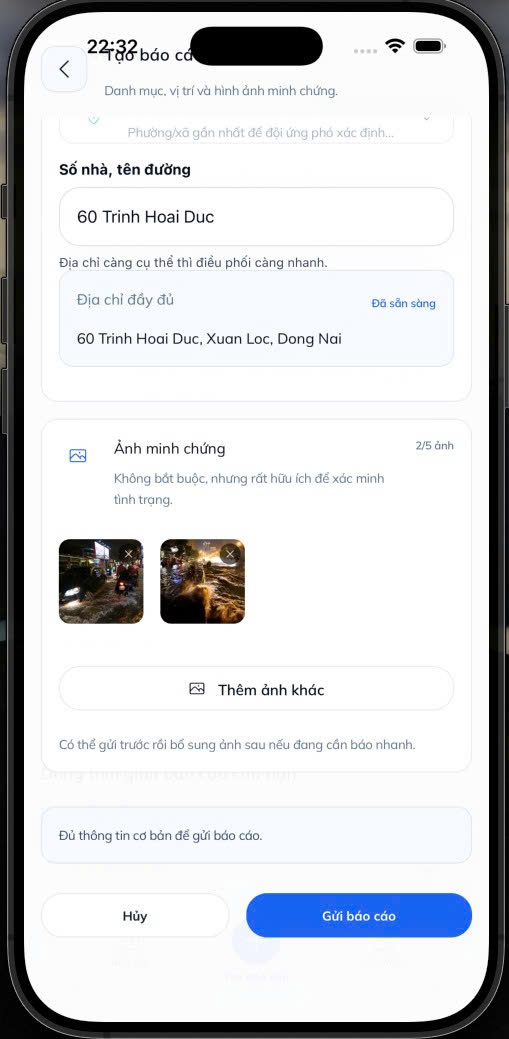
\includegraphics[width=0.38\linewidth,height=0.34\textheight,keepaspectratio]{images/figure2-4-mobile- evidence-upload.png.jpg}
    }{
        \fbox{
            \begin{minipage}[c][4.1cm][c]{0.38\linewidth}
                \centering
                Placeholder for Figure 2.3a\\[0.3cm]
                Suggested image: mobile evidence picker/upload UI.\\[0.2cm]
                File name:\\
                \texttt{figure2-4-mobile-}\\
                \texttt{evidence-upload.png.jpg}
            \end{minipage}
        }
    }
    \hfill
    \IfFileExists{images/figure2-4-dashboard-relief-evidence-review.jpg}{
        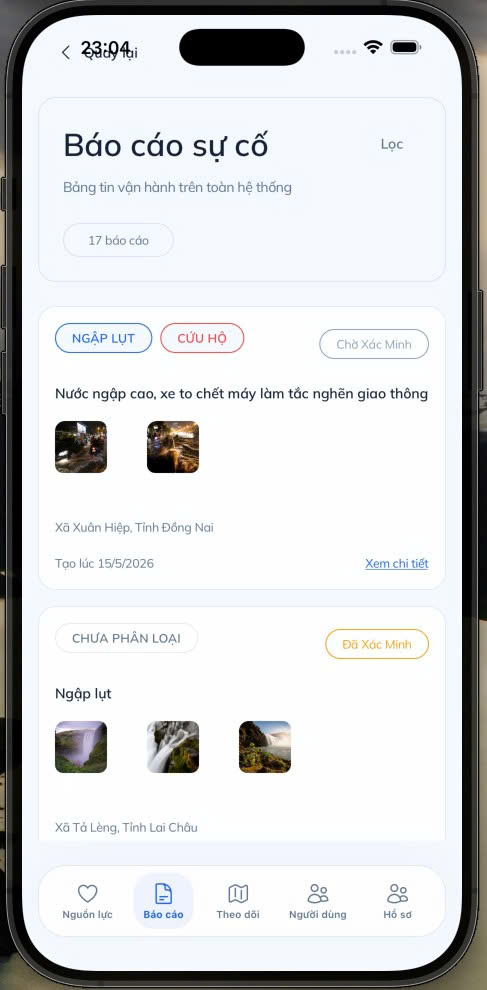
\includegraphics[width=0.52\linewidth,height=0.34\textheight,keepaspectratio]{images/figure2-4-dashboard-relief-evidence-review.jpg}
    }{
        \fbox{
            \begin{minipage}[c][4.1cm][c]{0.52\linewidth}
                \centering
                Placeholder for Figure 2.3b\\[0.3cm]
                Suggested image: dashboard evidence review UI.\\[0.2cm]
                File name:\\
                \texttt{figure2-4-dashboard-relief-}\\
                \texttt{evidence-review.jpg}
            \end{minipage}
        }
    }
    \caption{Example views of evidence upload on mobile and evidence review on the dashboard.}
    \label{fig:chapter2-evidence-examples}
\end{figure}

\subsection{Redis Cache Layer}

Redis is used as a cache layer to reduce repeated reads for frequently requested report details \cite{redisDocs}. Caching is kept conservative in the prototype. PostgreSQL remains the source of truth, while Redis stores temporary copies that can be refreshed after report updates. This design avoids complex cache invalidation rules while still demonstrating a realistic backend optimization approach.

\section{Access Control and Real-Time Channels}

\subsection{JWT Tokens and Password Hashing}

Role-based access control requires reliable authentication. VietFlood uses bcrypt hashing for passwords \cite{provos1999bcrypt} and JWT access tokens for stateless verification of identity and role claims \cite{jones2015jwt}. Refresh tokens are used to maintain longer sessions while allowing access tokens to remain short-lived.

\subsection{Socket.IO for Live Location Updates}

Real-time communication can support situational awareness when users share location updates. VietFlood includes a Socket.IO gateway for live location broadcasting \cite{socketioDocs}. The prototype validates coordinate ranges and broadcasts events between connected clients. This provides a minimal foundation for live tracking without expanding scope into persistent tracking histories or assignment workflows.

\section{Deployment and Environment Repeatability}

Repeatable environments are important even for prototypes. VietFlood uses Docker Compose to run backend services and infrastructure dependencies locally \cite{dockerComposeDocs}. The deployment approach follows standard CI/CD practices: images can be built and deployed automatically using GitHub Actions and Azure App Service container deployment \cite{githubActionsDocs,azureAppServiceContainersDocs}. Continuous delivery guidance motivates keeping build and deployment steps repeatable and automated rather than relying on manual server setup \cite{humble2010continuousDelivery,kim2016devopsHandbook}.
